\section{Wprowadzenie}
\subsection{Cel projektu}
Celem projektu było zastosowanie algorytmu ewolucyjnego w grze Othello.

\subsection{Opis gry Othello}
Othello jest grą planszową dla dwóch graczy, rozgrywaną na planszy o wymiarach 8 na 8 pól za pomocą 64 białych i czarnych pionów. Celem gry jest wypełnienie planszy większą liczbą własnych pionów niż przeciwnik. Rozgrywka rozpoczyna się od stanu, w którym na planszy są ustawione dwa piony czarne i dwa białe, w sposób przedstawiony na poniższym rysunku. Pierwszy ruch wykonuje rozgrywający piony czarne. Jedyne dozwolone ruchy polegają na otaczaniu i zdobywaniu pionów przeciwnika. Piony przeciwnika zdobywa się, otaczając je w jednej linii (pionowo, poziomo lub skośnie). Zdobyte piony zmieniają kolor i przynależność. W każdym ruchu należy zdobyć co najmniej jeden pion przeciwnika. Jeśli gracz nie może wykonać żadnego dozwolonego ruchu, traci kolejkę i wykonuje go drugi gracz. Gra kończy się, gdy żaden z graczy nie może już wykonać poprawnego ruchu.
\begin{figure}[h!]
\centering
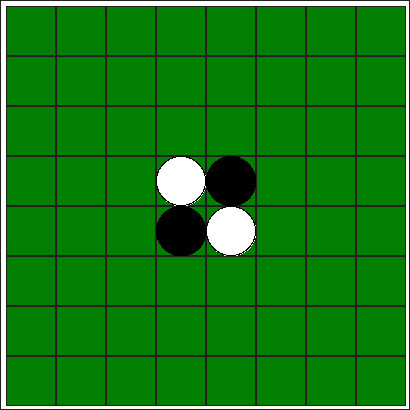
\includegraphics[scale=0.5]{img/othello_start.png}
\caption{Układ pionów przy rozpoczęciu gry.} 
\end{figure}
